\subsubsection{Curvature}

\begin{figure}[H]
    \begin{subfigure}[t]{0.47\textwidth}
        \scalebox{0.9}{%
        \begin{tikzpicture}
\begin{axis}[xmin=-0.7,
             xmax=0.7,
             ymin=-0.1,
             ymax=1.1,
             samples=200,
             axis line style={draw=none},
             tick style={draw=none},
             xticklabels={\empty},
             yticklabels={\empty},
             grid=major,
             plot box ratio={2 1},
             axis equal]
    \draw[plotorange, line width=1.3pt] (axis cs:0,0.5) circle [radius=50];
    \addplot[plotblue, line width=1.5pt] {x*x};
    \coordinate (C) at (axis cs:{0.0,0.5});
    \coordinate (O) at (axis cs:{0.0,0.0});
    \coordinate (L) at (axis cs:{0.1,0.25});
    \node at (L) {$\mathbf{r}$};
    \node[label={90:{$\mathbf{C}$}},circle,fill,inner sep=1pt] at (C) {};
    \draw[thick,-](C)--(O);
\end{axis}
\end{tikzpicture}

        }
        \caption{The curvature of a line at a specific point is defined through its osculating circle.}
    \end{subfigure}
    \begin{subfigure}[t]{0.47\textwidth}
        \scalebox{0.9}{%
        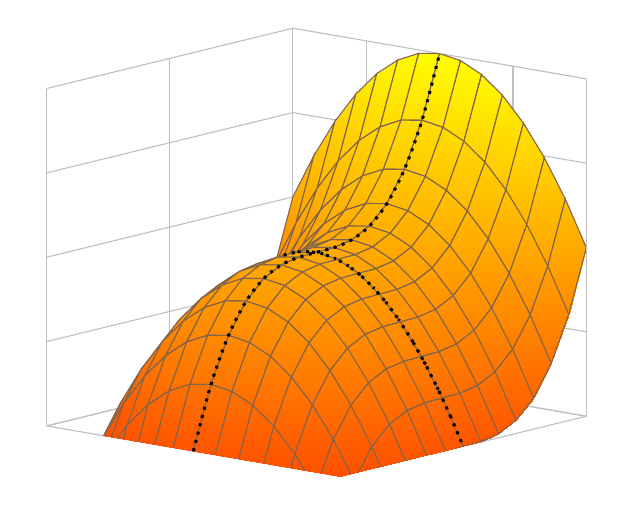
\begin{tikzpicture}
\begin{axis}[xmin=-1.0,xmax=1.0,
             ymin=-1.0,ymax=1.0,
             zmin=-1.0,zmax=1.0,
             grid=major,
             axis line style={draw=none},
             tick style={draw=none},
             view={310}{35},
             xticklabels={\empty},
             yticklabels={\empty},
             zticklabels={\empty},
             plot box ratio={1 1 3},
             colormap/redyellow]
\newcommand\func[2]{#1^3 - #2^2}
\definecolor{darkorange}{HTML}{84644B}

    \addplot3[surf,
              shader=faceted interp,
              faceted color={darkorange},
              samples=15,
              domain=-1:1,
              y domain=-1:1] {\func{x}{y}};

    % plot curve for x direction
    \addplot3[samples=15,
              domain=-1:1,
              samples y=1,
              dotted,
              black,
              line width=1.1pt,
              smooth] (x, 0, \func{x}{0});
    % plot curve for y direction
    \addplot3[samples=15,
              domain=-1:1,
              y domain=-1:0.22,
              dotted,
              black,
              line width=1.1pt,
              smooth] (0, y, \func{0}{y});
\end{axis}
\end{tikzpicture}

        }
        \caption{The curvature of a surface at a given point depends on the direction of measurement. The principal curvatures are the maximum and minimum value of curvatures in all directions.}
    \end{subfigure}
\end{figure}

As a different analytical approach to producing feature images the calculation of the \gls{curvature} for each depth value.
The two common measures of curvature in differential geometry are \gls{gaussian-curvature} and \gls{mean-curvature}\cite{Kuhnel2008}.

If the function is known as a graph the \Gls{gaussian-curvature} can be estimated using the derivatives of the function.
For depth data each depth value is a sample of this function graph and numeric approximation of the derivatives allows the calculation of the curvature.
\begin{align}
    \mathfrak{K} &= \frac{f_{uu} f_{vv} - f_{uv}^2}{{(1 + f_u^2 + f_v^2)}^2}
\end{align}
With
\begin{align*}
    f_{x} &= \frac{y_1 - y_0}{\Delta x} \\
    f_{xx} &= \frac{y_1 + y_{-1} - 2 y_0}{{\Delta x}^2}
\end{align*}
as approximation for the derivatives.

Similarly, the \Gls{mean-curvature} can be calculated with a different formula.
\begin{align}
    \mathfrak{H} &= \frac{{(1 + f_{v}^2)} f_{uu} - 2 f_u f_v f_{uv} + {(1 + f_u^2)} f_{vv}}{2 \sqrt{1 + f_u^2 + f_v^2}^3}
\end{align}
Both measures of curvature are $\mathfrak{K},\mathfrak{H} \in {\rm I\!R}$.
To convert them into a meaningful grayscale image they need to be clamped to arbitrary bounds, that can be choosen based on visual distinctiveness or other heuristics.
After clamping the values are scaled and quantized accordingly.

\begin{figure}[H]
    \begin{subfigure}[t]{0.32\textwidth}
        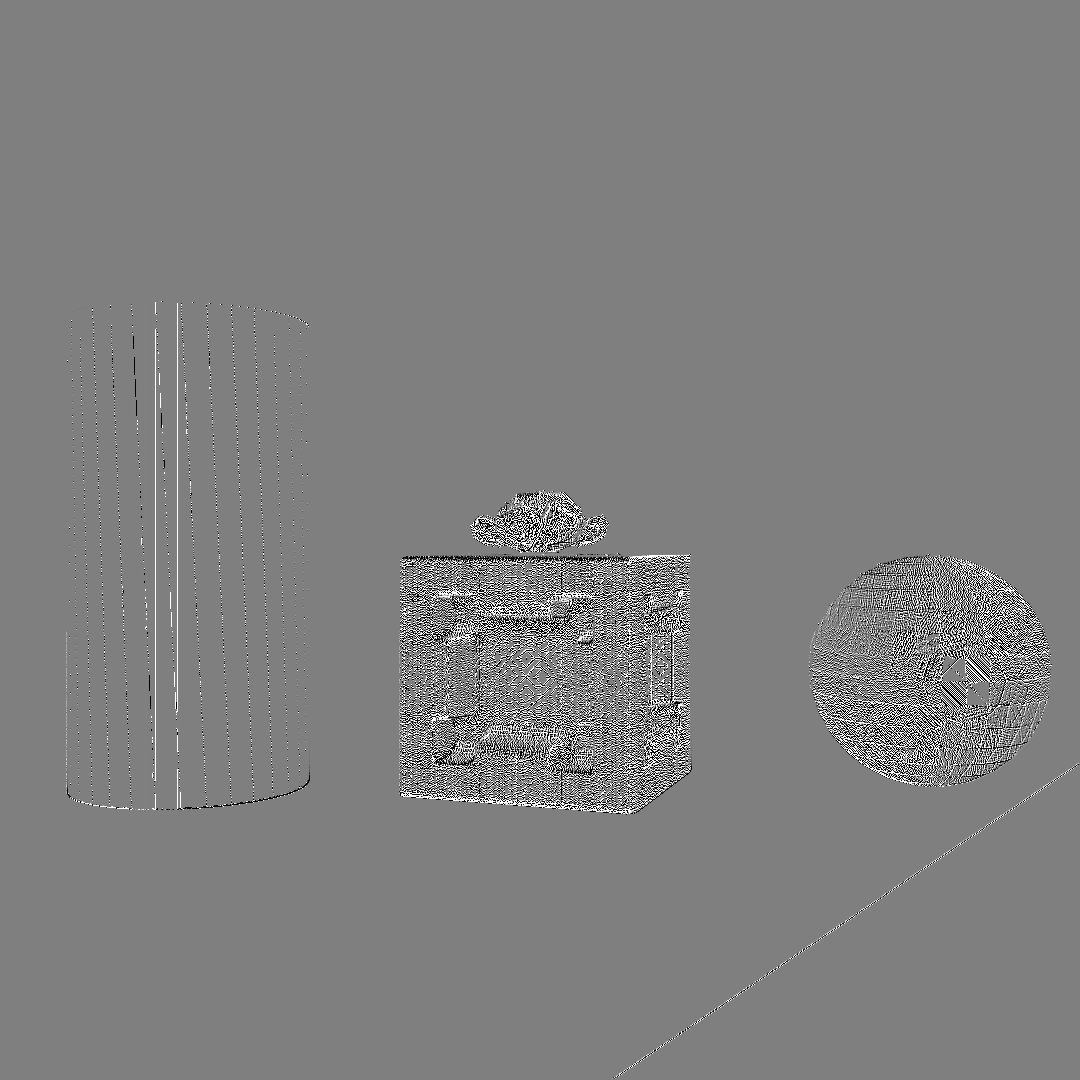
\includegraphics[width=\linewidth]{chapter04/img/mean-0001.png}
        \caption{This figure shows a converted \gls{bearing-angle-image} on a synthetic rendered scene.}
    \end{subfigure}
    \begin{subfigure}[t]{0.32\textwidth}
        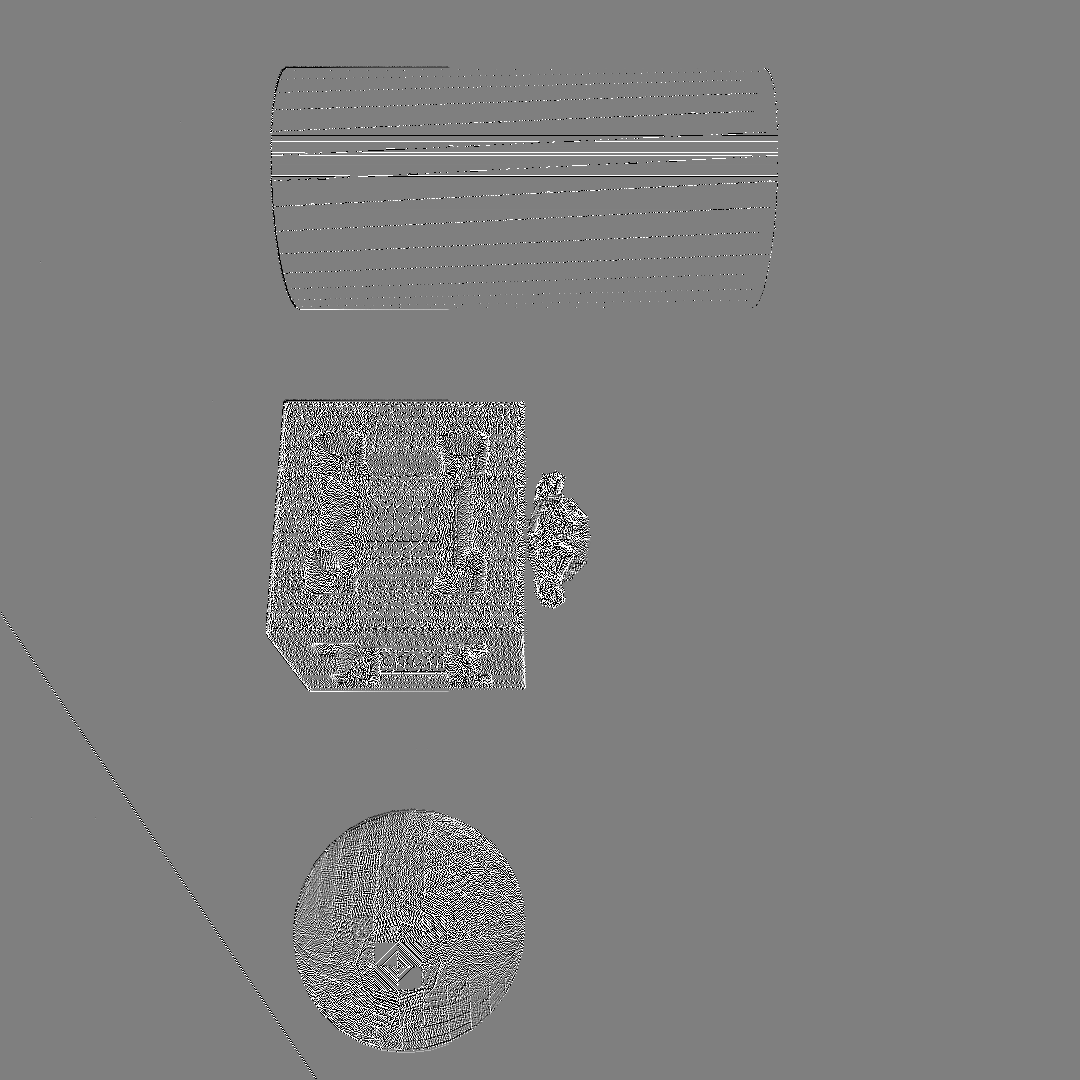
\includegraphics[width=\linewidth]{chapter04/img/mean-0030.png}
        \caption{Rotating the camera demonstrates color changes of surfaces.}
    \end{subfigure}
    \begin{subfigure}[t]{0.32\textwidth}
        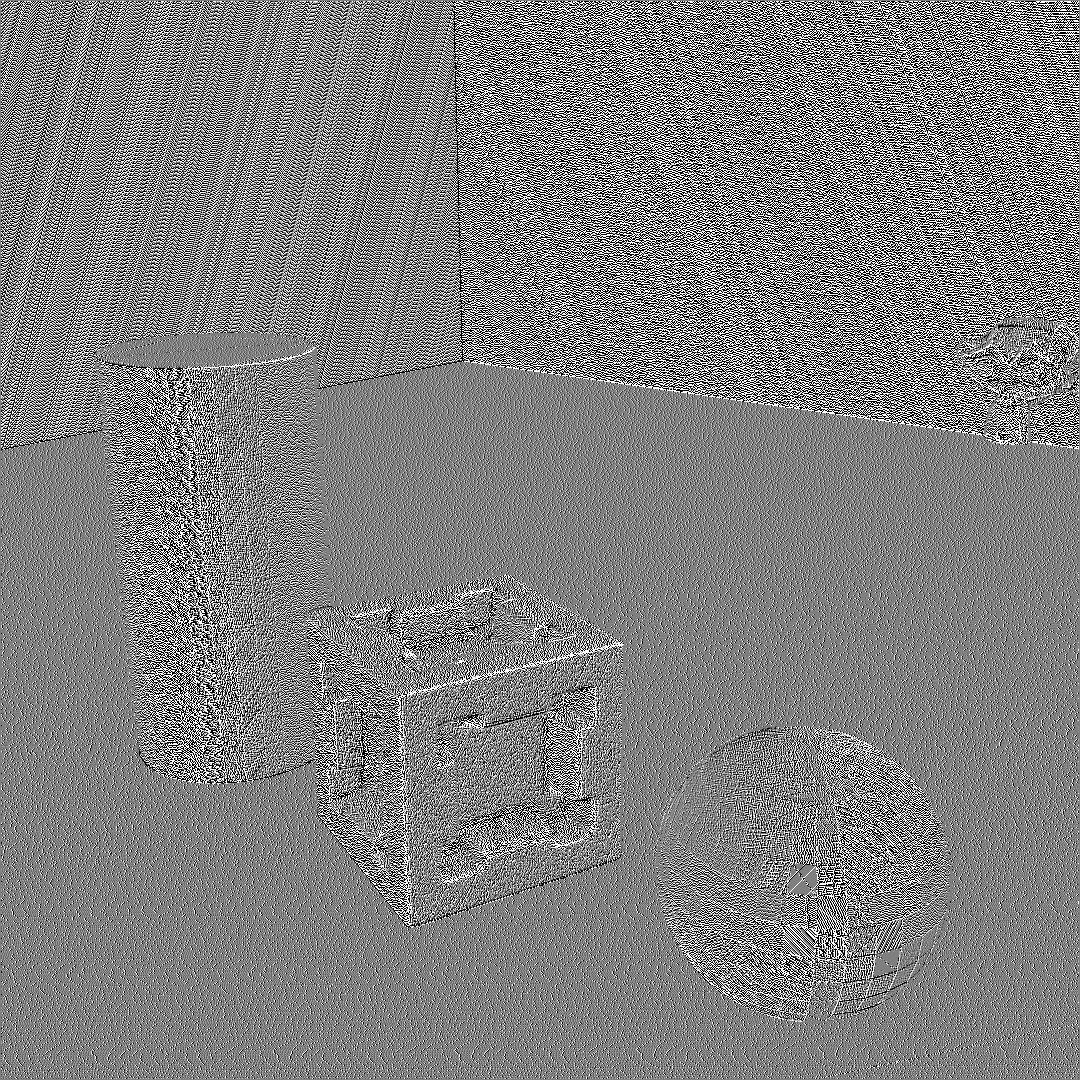
\includegraphics[width=\linewidth]{chapter04/img/mean-0210.png}
        \caption{A different camera pose result in different surface shading.}
    \end{subfigure}
\end{figure}


\begin{figure}[H]
    \begin{subfigure}[t]{0.32\textwidth}
        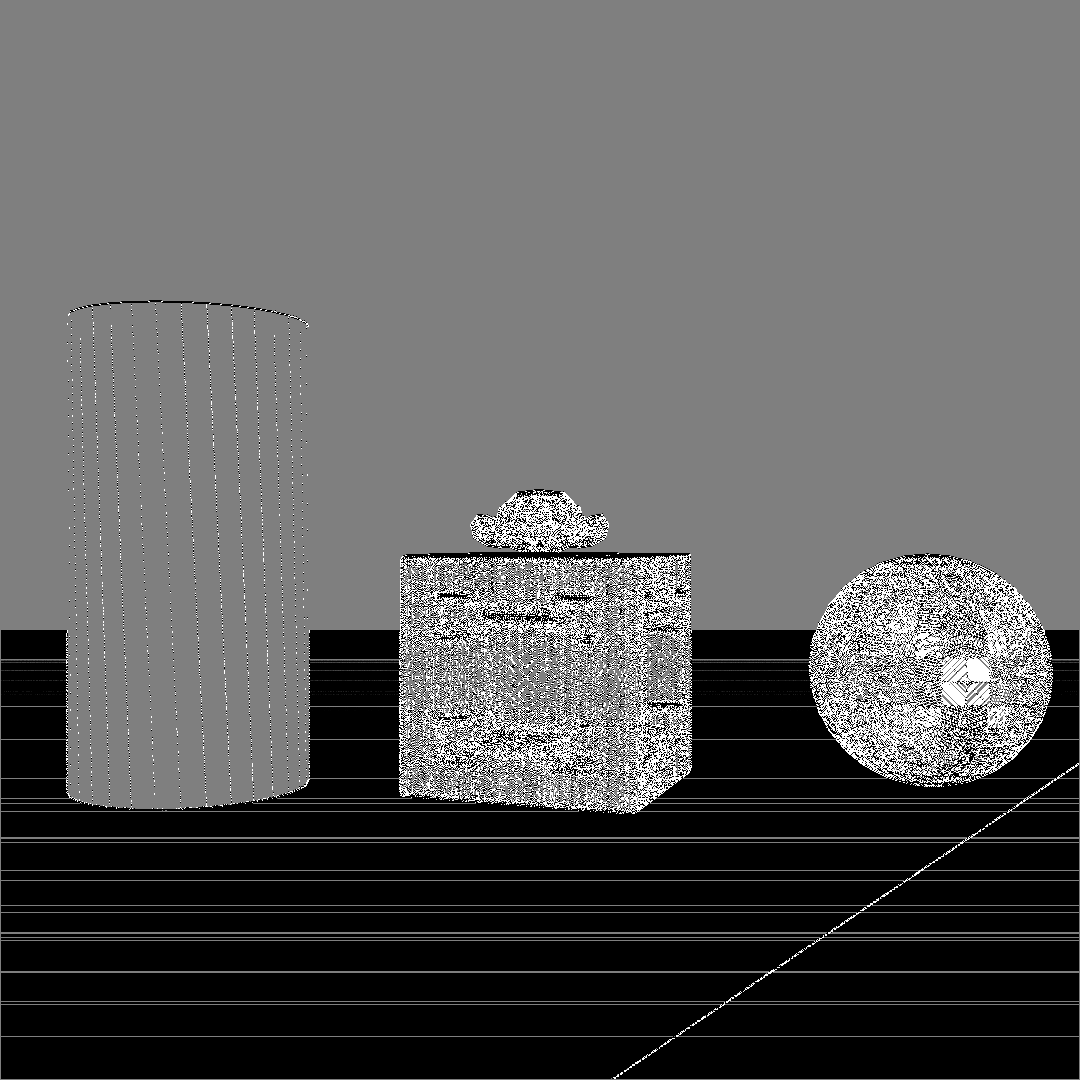
\includegraphics[width=\linewidth]{chapter04/img/gauss-0001.png}
        \caption{This figure shows a converted \gls{bearing-angle-image} on a synthetic rendered scene.}
    \end{subfigure}
    \begin{subfigure}[t]{0.32\textwidth}
        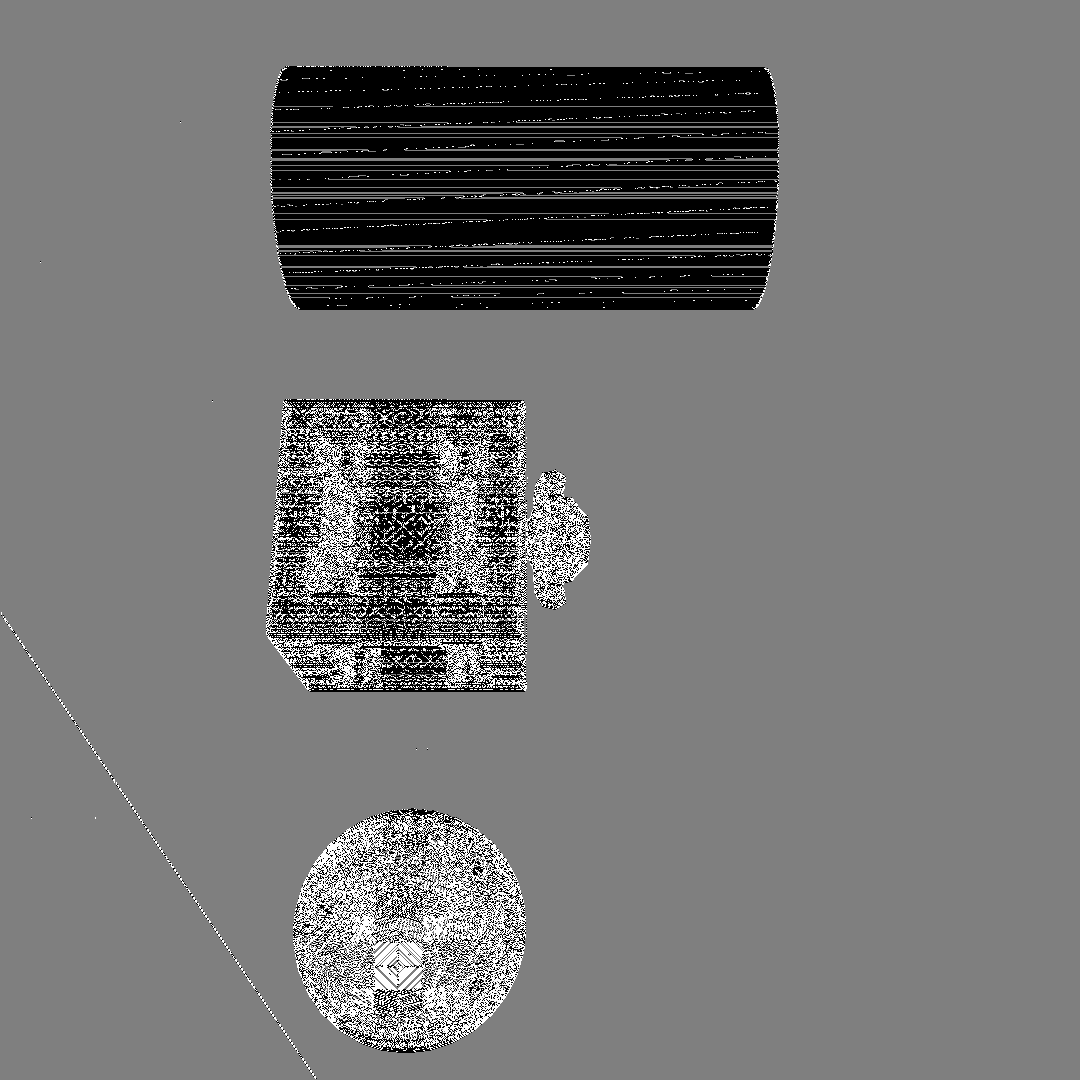
\includegraphics[width=\linewidth]{chapter04/img/gauss-0030.png}
        \caption{Rotating the camera demonstrates color changes of surfaces.}
    \end{subfigure}
    \begin{subfigure}[t]{0.32\textwidth}
        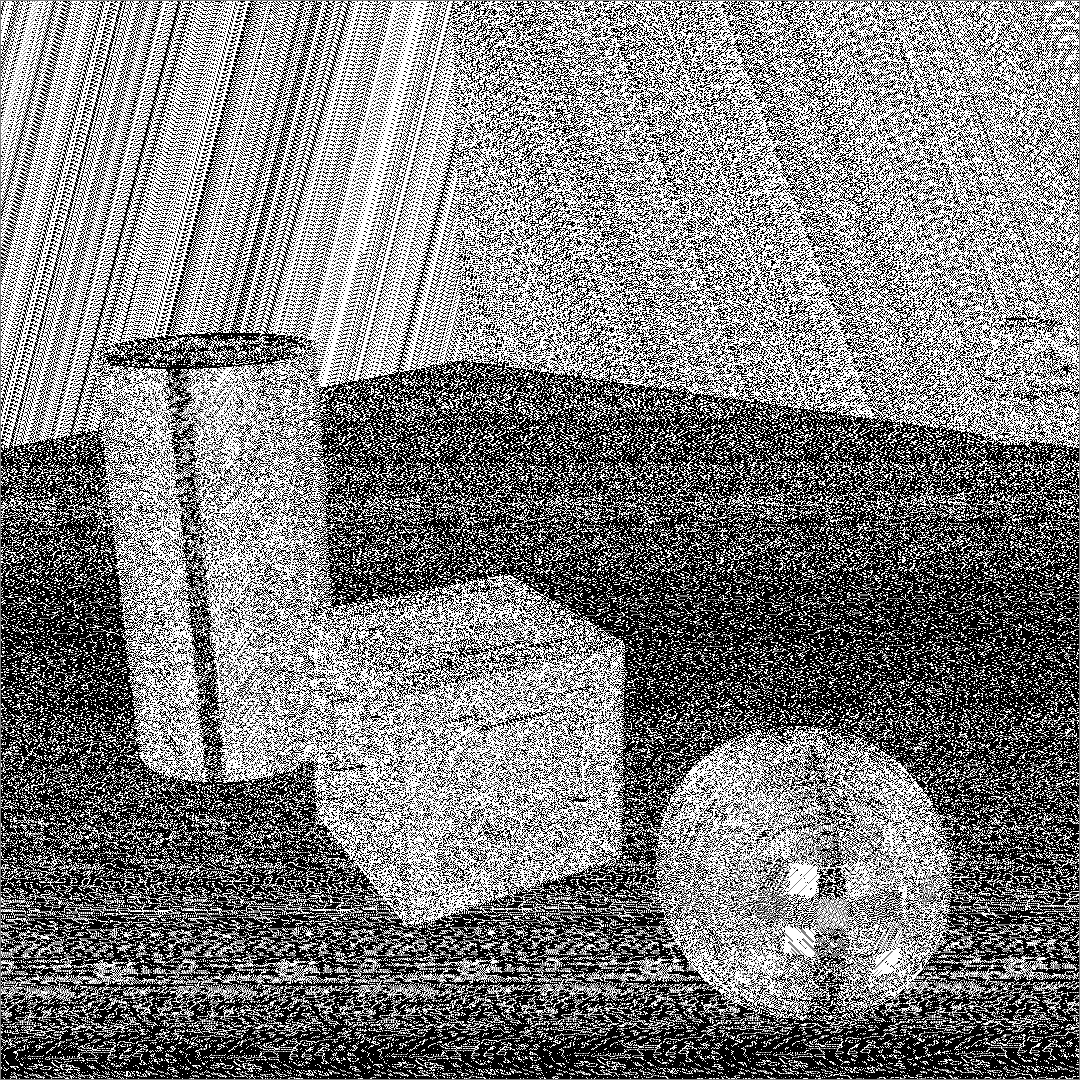
\includegraphics[width=\linewidth]{chapter04/img/gauss-0210.png}
        \caption{A different camera pose result in different surface shading.}
    \end{subfigure}
\end{figure}
